\documentclass[11pt]{article}
\usepackage{hyperref}  % links
\usepackage{graphicx}  % images
\usepackage{listings}  % code
\usepackage{authblk}  % author info

% Preamble
% Metadata
\title{API Usage and Security}
\author{Temuulen Erdenebulgan}
\affil{
Department of Computer Science\\
Luther College\\
Decorah, IA 52101\\
erdete01@luther.edu
}
\date{\today}

% Document body
\begin{document}
\maketitle

\begin{abstract}

    This paper provides an overview of how to use API effectively and explores best practices to secure API Key. The following paper consists of three sections. First, it explains the basic and advanced usage of API in modern days. Second, it explores different ways to secure JSON Tokens when a user requests API. 
\end{abstract}

\section{Introduction to API}

In today's emerging technological and information world, companies interact with their customers through a wide variety of different communication channels. These communication channels include face-to-face, telephone, email, voicemails, wireless communication, and internet collaborative sessions. For example, in 2019, Internet business statistics from Statista~\cite{Digital18:online} reveal that the number of people using internet services is increasing every year. 

When there is a proliferation of internet usage in today's world, one of the effective ways for companies to communicate with costumers and other companies is through Application Programming Interfaces (API). With the help of API, the world is more connected than ever before. One can use API and get the following benefits. For instance, 1) grow customers to products and services through API ecosystems, 2) drive innovation by capitalizing on the composition of different APIs, 3) improve the time-to-value and time-to-market for new products, and 4) improve integration with web APIs. Therefore, APIs have become a new of exposing business functionalities to the outside world. 

However, since there could be possibilities to use APIs for unethical purposes, security is one of the essentials. When a company exposes its APIs to the world, limitless innovative ideas may pop up and add value to the data. Therefore, the use of APIs will become more advanced in the future. 

\section{API Security}

Security is not an afterthought. It is an integral part of any development project. It starts with the design, development, testing, deployment, and monitoring phases. 
There are several authentication standards available to secure a JSON file such as API Keys, OAuth 2.0, JWT, and so on. According to the Forbes website, on average 30,000 new websites are hacked every day~\cite{30000Web65:online}. Therefore, since cybercrime is the greatest threat to every company in the world, one must learn good skills to protect websites from any threat.

\subsection{API Key}

An application programming interface key is a unique identifier used to authenticate a user, developer, or calling program to an API. Since the API key provides direct access to data, it functions the same as a password that a user of a web or mobile app provides to gain access to the same data. Therefore, API keys are not considered secure~\cite{Whyandwh4:online}. Once the key is stolen, it has no expiration, so it may be used indefinitely causing some problems.

However, when using API Key, one should try its best to hide API Key as much as possible from the server code. One of the ways to hide API Key from the server code is storing the API Key in a different environment variable \cite{dotenvnp6:online}. To do that, 1) install dotenv which loads environment variables from a .env file into process.env, 2) As early as possible in your application, write the next code

\begin{lstlisting}[caption=\texttt{Hiding API Key}, captionpos=b, frame=trbl, showstringspaces=false]
 npm install dotenv
 require('dotenv').config()
\end{lstlisting}

3) Finally, after the first 2 steps, one should create a new file called .env and connect it to the API Key. 
\begin{lstlisting}[caption=\texttt{Hiding API Key, Part 2}, captionpos=b,
frame=trbl, showstringspaces=false]
 .env file: API_KEY='enter api key'
 server file: set api_key to process.env.API_KEY;
\end{lstlisting}

Since it's a bad practice to store API Key in the server file, this process can help to hide API Key successfully from your server file. However, this does not mean hackers can't find the password.

\subsection{Token Based Authentication}

One of the other ways to use APIs is through JWT Token. JSON Web Token (JWT) defines a container to transport data between interested parties in JSON. JWT works the same way as OAuth 2.0; it became an IETF (Internet Engineering Task Force) Standard in May 2015. The main idea of JWT is to exchange information based on tokens within a limited time frame.


\begin{figure}[!htbp]
    \centering
    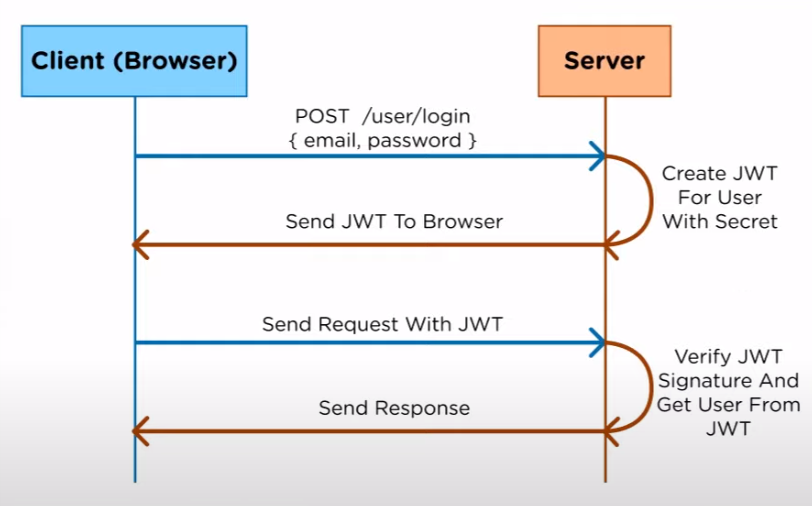
\includegraphics[width=1\textwidth]{Capture.PNG}
    \caption{JWET and JSON \cite{siriwardena2014advanced}}
    \label{fig:Capture}
\end{figure}


For instance, when the user successfully logs in using their credentials, a JSON Web Token, a string that the server generates for the client that can be passed along inside an HTTP request, with three main elements will be returned. Each element is base64url-encoded and separated by a period (.). After that, a client sends a request to the server; when a server receives a token, it can then look up the credentials of the user and determine whether or not it is authorized to the information.This makes it easier for the client application to exchange authentication credentials for authentication. Once authorized, JWT will decode base64url and make it readable for users \cite{JSONWebT36:online}.

Furthermore, tokens are usually given out with an expiration time after which they become 
invalid and a new token needs to be obtained. One can easily set a timer when building JWT; when the time exceeds, the token will no longer work.Therefore, the potential damage that can be caused if a token is stolen is low due to their short life span. 

Therefore, JWT is a very popular standard one can use to trust requests by using signatures, and exchange information between parties. 

\subsection{OAuth 2.0 Fundamentals}

OAuth 2.0 is the standard for securing APIs and is widely used by Facebook, Google, Spotify, Instagram, and many more. OAuth 2.0 solves access delegation problems without sharing user’s credentials with third-party applications. 

\begin{figure}[!htbp]
    \centering
    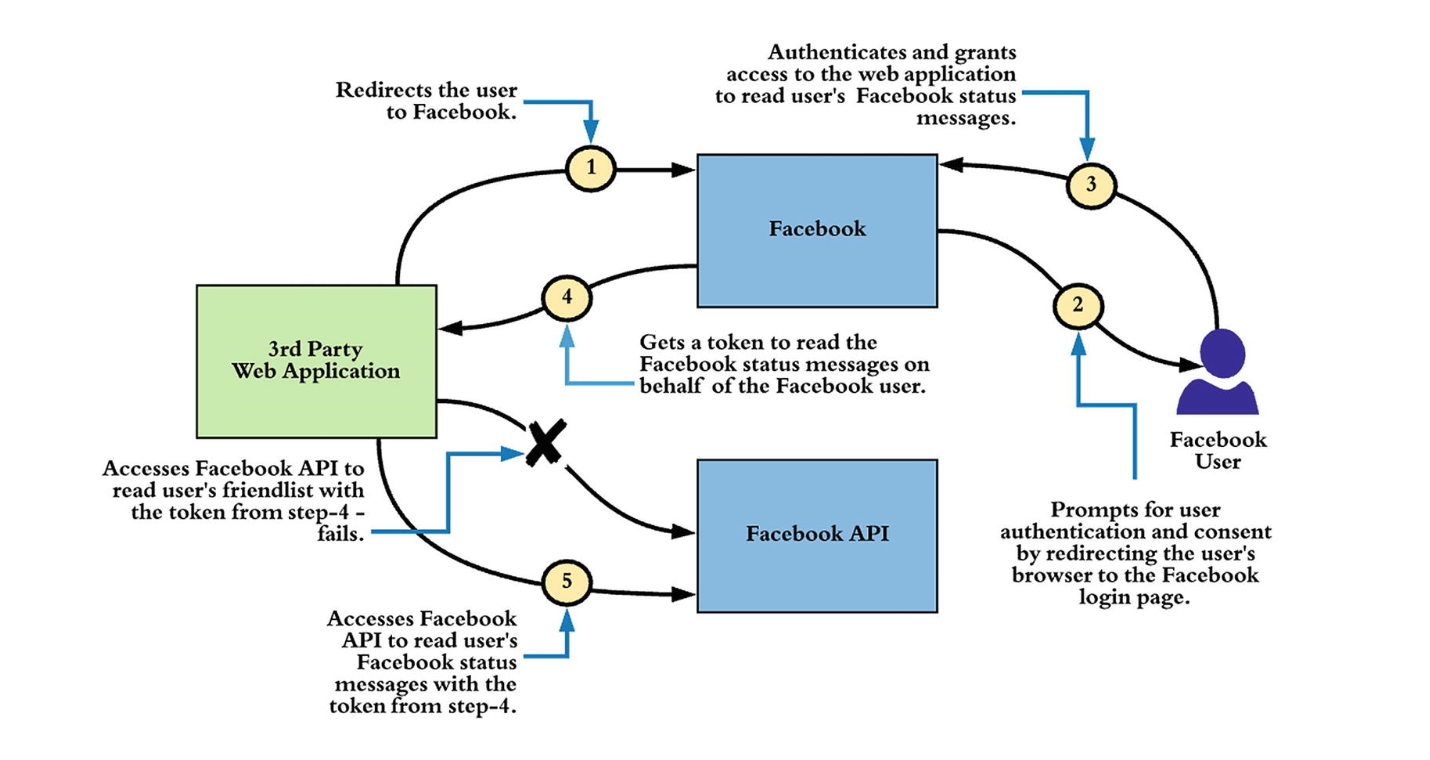
\includegraphics[width=1\textwidth]{facebok.PNG}
    \caption{OAuth 2.0 Example \cite{siriwardena2014advanced}}
    \label{fig:facebok}

\end{figure}

For example, when a user visits the third-party web application to publish messages to his/her Facebook wall, OAuth 2.0 gets the user token from Facebook and prompts the user to authenticate; requests consent from the user to give permissions to the third-part web application to publish messages to his/her Facebook wall. In this process, the third-party web application accesses the Facebook API with the token provided to it by Facebook without getting the user's password or any credentials. Only requesting a token from a server makes OAuth 2.0 useful for many cases.

OAuth 2.0 has advantages over a token-based authentication system or hashing passwords. Users had to authenticate a user based on their username and password or a token. But, to make a server that stores passwords have some drawbacks. For example, the user will be forced to make accounts, remember their passwords, and so on, it reduces the take more time for users to access the server. 

Therefore, OAuth 2.0 is a very popular tool because it helps the server to save so much time and used by many big companies such as Spotify, Google, and Facebook.

\section{Conclusion}
This paper explored an overview of how to use API more effectively. API is used for many different reasons such as retrieving data, communicating with users, and authenticating users. Furthermore, API has three different ways to secure a JSON Token. Those three ways are: calling API through API Key, accessing token based authentication, and using OAuth 2.0 methods.

\bibliographystyle{plain}
\bibliography{sources.bib}
\end{document}


